% Options for packages loaded elsewhere
\PassOptionsToPackage{unicode}{hyperref}
\PassOptionsToPackage{hyphens}{url}
%
\documentclass[
]{book}
\usepackage{amsmath,amssymb}
\usepackage{lmodern}
\usepackage{iftex}
\ifPDFTeX
  \usepackage[T1]{fontenc}
  \usepackage[utf8]{inputenc}
  \usepackage{textcomp} % provide euro and other symbols
\else % if luatex or xetex
  \usepackage{unicode-math}
  \defaultfontfeatures{Scale=MatchLowercase}
  \defaultfontfeatures[\rmfamily]{Ligatures=TeX,Scale=1}
\fi
% Use upquote if available, for straight quotes in verbatim environments
\IfFileExists{upquote.sty}{\usepackage{upquote}}{}
\IfFileExists{microtype.sty}{% use microtype if available
  \usepackage[]{microtype}
  \UseMicrotypeSet[protrusion]{basicmath} % disable protrusion for tt fonts
}{}
\makeatletter
\@ifundefined{KOMAClassName}{% if non-KOMA class
  \IfFileExists{parskip.sty}{%
    \usepackage{parskip}
  }{% else
    \setlength{\parindent}{0pt}
    \setlength{\parskip}{6pt plus 2pt minus 1pt}}
}{% if KOMA class
  \KOMAoptions{parskip=half}}
\makeatother
\usepackage{xcolor}
\IfFileExists{xurl.sty}{\usepackage{xurl}}{} % add URL line breaks if available
\IfFileExists{bookmark.sty}{\usepackage{bookmark}}{\usepackage{hyperref}}
\hypersetup{
  pdftitle={CASA0023 Remotely Sensing Cities and Environments},
  pdfauthor={Andy MacLachlan},
  hidelinks,
  pdfcreator={LaTeX via pandoc}}
\urlstyle{same} % disable monospaced font for URLs
\usepackage{longtable,booktabs,array}
\usepackage{calc} % for calculating minipage widths
% Correct order of tables after \paragraph or \subparagraph
\usepackage{etoolbox}
\makeatletter
\patchcmd\longtable{\par}{\if@noskipsec\mbox{}\fi\par}{}{}
\makeatother
% Allow footnotes in longtable head/foot
\IfFileExists{footnotehyper.sty}{\usepackage{footnotehyper}}{\usepackage{footnote}}
\makesavenoteenv{longtable}
\usepackage{graphicx}
\makeatletter
\def\maxwidth{\ifdim\Gin@nat@width>\linewidth\linewidth\else\Gin@nat@width\fi}
\def\maxheight{\ifdim\Gin@nat@height>\textheight\textheight\else\Gin@nat@height\fi}
\makeatother
% Scale images if necessary, so that they will not overflow the page
% margins by default, and it is still possible to overwrite the defaults
% using explicit options in \includegraphics[width, height, ...]{}
\setkeys{Gin}{width=\maxwidth,height=\maxheight,keepaspectratio}
% Set default figure placement to htbp
\makeatletter
\def\fps@figure{htbp}
\makeatother
\setlength{\emergencystretch}{3em} % prevent overfull lines
\providecommand{\tightlist}{%
  \setlength{\itemsep}{0pt}\setlength{\parskip}{0pt}}
\setcounter{secnumdepth}{5}
\usepackage{booktabs}
\ifLuaTeX
  \usepackage{selnolig}  % disable illegal ligatures
\fi
\usepackage[style=apa,]{biblatex}
\addbibresource{zotero.bib}

\title{CASA0023 Remotely Sensing Cities and Environments}
\author{Andy MacLachlan\footnote{The Bartlett Centre for Advanced Spatial Analysis, \url{https://twitter.com/andymaclachlan}}}
\date{2021-08-27}

\begin{document}
\maketitle

\hypertarget{welcome}{%
\chapter*{Welcome}\label{welcome}}
\addcontentsline{toc}{chapter}{Welcome}

Hello and welcome to the Term 2 module Remotely Sensing Cities and Environments.

Similarly, to my Term 1 MSc module, CASA0005, this website holds all the practical instructions for the module. \href{https://andrewmaclachlan.github.io/CASA0005repo/}{CASA0005 Geographic Information Systems and Science} is a pre-requisite of the module so concepts taught there will mainly be assumed here.

\hypertarget{acknowledgement}{%
\section*{Acknowledgement}\label{acknowledgement}}
\addcontentsline{toc}{section}{Acknowledgement}

Thanks to the following academics who inspired the creating of the module and various concepts within it:

\begin{itemize}
\tightlist
\item
  \href{https://twitter.com/EllieMBiggs}{Dr Ellie Biggs}
\item
  \href{https://www.southampton.ac.uk/geography/about/staff/gjr1f10.page}{Dr Gareth Roberts}
\item
  \href{https://directory.uwa.edu.au/view?dn=cn\%3DBryan\%20Boruff\%2Cou\%3DDepartment\%20of\%20Geography\%20and\%20Planning\%2Cou\%3DArts\%5C2C\%20Business\%5C2C\%20Law\%20and\%20Education\%2Cou\%3DCollege\%20of\%20Schools\%2Co\%3DThe\%20University\%20of\%20Western\%20Australia}{Dr Bryan Boruff}
\item
  \href{https://www.southampton.ac.uk/geography/about/staff/ejm.page}{Professor Ted Milton}
\item
  \href{https://scholars.uow.edu.au/display/laurie_chisholm}{Dr Laurie Chisholm}
\end{itemize}

Thanks again to the following people who have either contributed directly or provided code in repositories that have helped me style this book:

\begin{itemize}
\tightlist
\item
  \href{https://stat545.com/index.html\#other-contributors}{STAT 545}
\item
  \href{https://rstudio4edu.github.io/rstudio4edu-book/}{rstudio4edu}
\item
  \href{https://twitter.com/hadleywickham}{Hadley Wickham}
\item
  \href{https://twitter.com/apreshill}{Alison Presmanes Hill}
\item
  \href{https://twitter.com/dcossyle}{Desirée De Leon}
\item
  \href{https://twitter.com/xieyihui}{Yihui Xie}
\item
  \href{https://twitter.com/robinlovelace}{Robin Lovelace}
\item
  \href{https://www.t4rstats.com/index.html}{Twitter for R programmers}
\item
  \href{https://twitter.com/mattnkm}{Matt Ng}
\item
  \href{https://www.youtube.com/channel/UCtYLUTtgS3k1Fg4y5tAhLbw}{StatQuest with Josh Starmer}
\item
  \href{https://twitter.com/juliasilge}{Julia Silge}
\item
  \href{https://twitter.com/JennyBryan}{Jenny Bryan}
\item
  \href{https://twitter.com/grrrck}{Garrick Aden‑Buie}
\end{itemize}

The R package and analysis artwork used within this book has been produced by \href{https://twitter.com/allison_horst}{allison\_horst}, whilst artwork used in information boxes has been produced by \href{https://twitter.com/dcossyle}{Desirée De Leon}. You can find Allison's images on the \href{https://github.com/allisonhorst/stats-illustrations}{stats illustration GitHub repository} and Desirée's on the \href{https://github.com/rstudio4edu/rmd4edu}{rstudio4edu GitHub repository}.

I've certainly learnt a lot from their open code repositories!

\hypertarget{part-course-information}{%
\part*{Course information}\label{part-course-information}}
\addcontentsline{toc}{part}{Course information}

\hypertarget{hello-remote-sensing}{%
\chapter*{Hello Remote Sensing}\label{hello-remote-sensing}}
\addcontentsline{toc}{chapter}{Hello Remote Sensing}

Earth Observation can yield fascinating insights into geographical relationships. However, at times it can be difficult to work with. You will get lots of error messages and have software crash. The academic staff are here to help you work through these practicals but we do not know everything. It's a good idea to become familiar with online sources of help, such as:

\begin{itemize}
\tightlist
\item
  \href{https://stackexchange.com/}{Stack Exchange}
\item
  \href{https://community.rstudio.com/}{RStudio community}
\item
  \href{https://docs.qgis.org/3.4/en/docs/index.html}{QGIS documemtation}
\item
  \href{https://www.rdocumentation.org/}{R documentation}
\item
  \href{https://support.esri.com/en}{ArcGIS help pages}
\end{itemize}

\hypertarget{learning-outcomes}{%
\section*{Learning outcomes}\label{learning-outcomes}}
\addcontentsline{toc}{section}{Learning outcomes}

At the end of this module you should be able to:

\begin{itemize}
\item
  Create a reproducible online portfolio workbook
\item
  Explain and evaluate common issues with urban and environmental policies at the local, national and international level that fail to consider spatial data
\item
  Revise vague and ambiguous development targets
\item
  Appropriately pre-process Earth observation imagery ready for analysis
\item
  Apply published methodologies to extract meaning from Earth observation data
\item
  Combine a variety of spatial data to demonstrate the benefits of data-informed governance and planning.
\item
  Create and design a reproducible workflow for consistent monitoring of urban and environmental metrics
\item
  Critique and optimise recently developed metropolitan climate mitigation strategies using appropriate spatial data, optimizing financial investment and environmental outcomes
\end{itemize}

\begin{infobox}{note}
There is a lot of information within this practical book and \textbf{we do not expect you to read everything we link to}. You should attend each lecture, go through every practical and do some associated reading.

This is a 15 credit module, equivalent to 150 hours of study (including the taught sessions). Outside of our lectures and practical sessions (4 hours a week) \textbf{you should be spending an extra 11 hours a week on this module}.

\end{infobox}

\hypertarget{how-to-use-this-book}{%
\section*{How to use this book}\label{how-to-use-this-book}}
\addcontentsline{toc}{section}{How to use this book}

To get the most out of this book spend a few minutes learning how to control it, in the top right of this webpage you will see this tools bar:

\begin{center}
\includegraphics[width=600pt]{general_images/Book_controls} \end{center}

From left to right these buttons will let you:

\begin{itemize}
\item
  control the side bar
\item
  search the entire book for a specific word
\item
  change the text size, font, colour
\item
  propose an edit if you see a mistake that I can review
\item
  view the webpage in the `raw' RMarkdown format, we cover RMarkdown in the course
\item
  information about shortcuts for this book and most others like it
\end{itemize}

In addition the icon in the top right of the page takes you to the GitHub repository for this book, we cover GitHub in the course, but it's basically where the online files for the book are stored.

\hypertarget{getting-started}{%
\section*{Getting started}\label{getting-started}}
\addcontentsline{toc}{section}{Getting started}

One of the issues with Remote Sensing is that many of the files we will be working with are quite large. Fortunately in recent years UCL has seriously beefed up the storage available for students. You now get 100GB of free storage, which should be plenty for the work you will be doing this year! The Bartlett faculty has several gigabytes of storage space available on their central servers, so before we get started, we will connect to our N drive to carry out all of our practical work over the coming weeks.

\begin{infobox}{note}
The data we use in this practical book is representative of what you will find when conducting independent analysis. Some books and website will give you perfectly `clean' and `ready to use' data, we have not done this on purpose as it's very important to master data wrangling (also called data manipulation). In the `real world' data is messy and it's vital you know how to deal with it. Take this quote from the \href{https://www.nytimes.com/2014/08/18/technology/for-big-data-scientists-hurdle-to-insights-is-janitor-work.html}{New York Times} for example\ldots{}

\emph{``Data scientists, according to interviews and expert estimates, spend from 50 percent to 80 percent of their time mired in this more mundane labor of collecting and preparing unruly digital data, before it can be explored for useful nuggets.''}

\end{infobox}

\hypertarget{how-to-download-data-and-files-from-github}{%
\section*{How to download data and files from GitHub}\label{how-to-download-data-and-files-from-github}}
\addcontentsline{toc}{section}{How to download data and files from GitHub}

The majority of data required for the workshops is found online and we detail how to download this within the workshops. On occasion you may need to get some data from my GitHub, the workshops will instruct you to do this where needed.

To do so you have a few options. Option 1 will let you download just a spceific folder whilst option 2 will download everything i have used to make the workshops.

\hypertarget{option-1}{%
\subsection*{Option 1}\label{option-1}}
\addcontentsline{toc}{subsection}{Option 1}

Use \href{https://minhaskamal.github.io/DownGit/\#/home}{DownGit}

\begin{enumerate}
\def\labelenumi{\arabic{enumi}.}
\item
  Go to: \url{https://minhaskamal.github.io/DownGit/\#/home}
\item
  Head over to the GitHub repository: \url{https://github.com/andrewmaclachlan/CASA0005repo}
\item
  Select a folder you wish to download --- here i'll use practical data as the example, click into the folder (prac7\_data) and copy the url: \url{https://github.com/andrewmaclachlan/CASA0005repo/tree/master/prac7_data}
\item
  Paste it into DownGit and click Download, once downloaded then unzip the folder.
\end{enumerate}

\hypertarget{option-2}{%
\subsection*{Option 2}\label{option-2}}
\addcontentsline{toc}{subsection}{Option 2}

\begin{enumerate}
\def\labelenumi{\arabic{enumi}.}
\item
  Go to the online repository page here: \url{https://github.com/andrewmaclachlan/CASA0005repo}
\item
  Click Clone or download, the download as ZIP. This will download the everything i have used to make this website including all the data for the practicals
\end{enumerate}

\begin{center}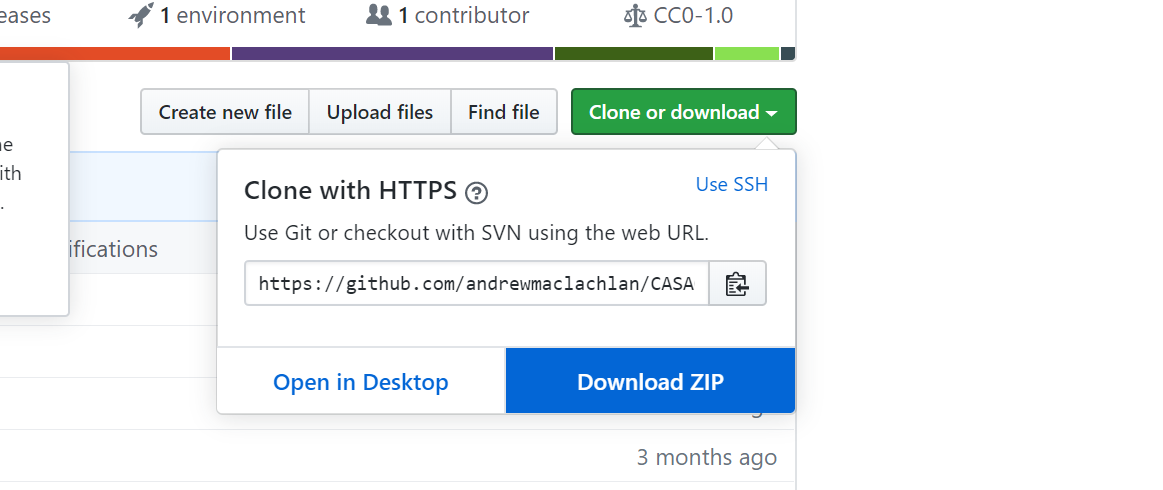
\includegraphics[width=500pt]{index_images/downloadrepo} \end{center}

\hypertarget{self-guided-learning}{%
\section*{Self guided learning}\label{self-guided-learning}}
\addcontentsline{toc}{section}{Self guided learning}

The lectures and practicals of this course only form a part of the learning process. You are expected to undertake wider reading and explore new methods and approaches. We have provided guidance on useful resources throughout the course to use as a starting point but you are encouraged to go beyond our recommedations and fully engage with applied GIS research, methods and visualisation techniques.

If you find a practical particularly easy or straightforward then please move on to the next one. Practicals that look at analytical relationships also have extension activities for you to try.

\hypertarget{interactive-lectures}{%
\section*{Interactive lectures}\label{interactive-lectures}}
\addcontentsline{toc}{section}{Interactive lectures}

During the lectures we will be using an interative polling and Q\&A application called vevox. It's very simple to use, you can either:

\begin{itemize}
\tightlist
\item
  Download the app on iOS or Android: \url{http://get.vevox.app}
\item
  Use the web app: \url{https://vevox.app/}
\end{itemize}

The meeting ID we will use is: 186-395-009

\hypertarget{more-help}{%
\section*{More help}\label{more-help}}
\addcontentsline{toc}{section}{More help}

If you need specific assistance with this course please:

\begin{itemize}
\item
  Check the Moodle assessment tab for queries relating to assignments / deadlines.
\item
  Speak to a member of the teaching team in the computer lab sessions
\item
  Ask a question at the end of a lecture (time permitting)
\item
  Ask a question on slack under the Remote Sensing channel
\end{itemize}

Due to the size of the class we will \textbf{only reply} to messages \textbf{on slack} so all students can see the discussion. If you have a personal matter in relation to completing the course then please speak to or email Andy

\hypertarget{noticed-a-mistake}{%
\section*{Noticed a mistake?}\label{noticed-a-mistake}}
\addcontentsline{toc}{section}{Noticed a mistake?}

No one is perfect, if you notice a mistake let us know through the \href{https://github.com/andrewmaclachlan/CASA0005repo/issues}{GitHub issues tab}

Don't worry if you are unsure about what GitHub is we cover it in the course.

\hypertarget{assignment-resources}{%
\section*{Assignment resources}\label{assignment-resources}}
\addcontentsline{toc}{section}{Assignment resources}

Want some tips for resources on your assignment?\ldots. head over to the \protect\hyperlink{assignment-resources}{Assignment resources} pages

\hypertarget{reading-list}{%
\section*{Reading list}\label{reading-list}}
\addcontentsline{toc}{section}{Reading list}

We link to books and resources throughout each practical and in the \protect\hyperlink{assignment-resources}{Assignment resources} pages.

\hypertarget{external-usage}{%
\chapter*{External usage}\label{external-usage}}
\addcontentsline{toc}{chapter}{External usage}

\hypertarget{how-to-adopt-this-course}{%
\section*{How to adopt this course}\label{how-to-adopt-this-course}}
\addcontentsline{toc}{section}{How to adopt this course}

All the required data to run this course or individual practicals is provided in the GitHub repository.

There are two main options to adopt this course:

\begin{enumerate}
\def\labelenumi{\arabic{enumi}.}
\item
  Adopt the course in its entirety by forking the repository on GitHub and Pulling to your local machine or simply download a \texttt{.zip} file containing the entire course.
\item
  Adopt a single practical by downloading the \texttt{.rmd} file and associated data.
\end{enumerate}

Instructions can be found in the section \protect\hyperlink{how-to-download-data-and-files-from-github}{How to download data and files from GitHub}

\hypertarget{issues-contributions}{%
\section*{Issues / contributions}\label{issues-contributions}}
\addcontentsline{toc}{section}{Issues / contributions}

To raise an issue simply log it on the \href{}{GitHub issues tab for the repository}.

To propose an edit click on the edit symbol in the top tool bar (see \protect\hyperlink{how-to-use-this-book}{How to use this book}) and submit it for review.

If you wish to contribute material or data then please contact the course convenor Andy MacLachlan (details below).

\hypertarget{license}{%
\section*{License}\label{license}}
\addcontentsline{toc}{section}{License}

If you use this material for teaching, research or anything else please let me (Andy) know via \href{https://twitter.com/andymaclachlan}{Twitter} or email --- a {[}dot{]} maclachlan {[}at{]} ucl {[}dot{]} ac {[}dot{]} uk).

This practical book is licensed under a \href{https://creativecommons.org/licenses/by-sa/4.0/}{Creative Commons Attribution-ShareAlike 4.0 International (CC BY-SA 4.0) License}.

You are free to:

\begin{itemize}
\item
  \textbf{Share} --- copy and redistribute the material in any medium or format
\item
  \textbf{Adapt} --- remix, transform, and build upon the material
  for any purpose, even commercially.
\end{itemize}

However, you give appropriate credit, provide a link to the license, and indicate if changes were made. If you remix, transform, or build upon the material, you must distribute your contributions under the same license as the original.

But, you do not have to comply with the license for elements of the material in the public domain or where your use is permitted by an applicable exception or limitation.

The code within this practical book is available under the \href{https://opensource.org/licenses/MIT}{MIT license}; so it is free to use (for any purpose) as long as you cite the source.

\hypertarget{version}{%
\section*{Version}\label{version}}
\addcontentsline{toc}{section}{Version}

This is version 1.0 of the practical book

\hypertarget{part-remote-sensing}{%
\part{Remote Sensing}\label{part-remote-sensing}}

\hypertarget{remote-sensing-101}{%
\chapter{Remote Sensing 101}\label{remote-sensing-101}}

\hypertarget{learning-outcomes-1}{%
\section{Learning outcomes}\label{learning-outcomes-1}}

By the end of this practical you should be able to:

\begin{enumerate}
\def\labelenumi{\arabic{enumi}.}
\tightlist
\item
\item
\end{enumerate}

\hypertarget{homework}{%
\section{Homework}\label{homework}}

Outside of our scheduled sessions you should be doing around 11 hours of extra study per week. Feel free to follow your own interests, but good places to start include the following:

\begin{infobox}{note}
\textbf{Workbook}

Each week you need to write a response to the workbook questions

\end{infobox}

\begin{infobox}{note}

\textbf{Reading}

\begin{itemize}
\tightlist
\item
  Landsat: Building a strong future, \textcite{lovelandLandsatBuildingStrong2012}
\item
  Global science for city policy, \textcite{MicheleAcuto2018}
\item
  \href{https://earthdata.nasa.gov/learn/backgrounders/remote-sensing}{NASA remote sensing background}
\end{itemize}

\textbf{Watching}

\begin{itemize}
\tightlist
\item
  \href{https://www.youtube.com/watch?v=N49PzLDUIFQ}{What is remote sensing}
\end{itemize}

\end{infobox}

Within this first practical we are going to focus on loading and manipulating remotely sensed data and exploring the different resolutions

\hypertarget{cross}{%
\chapter{Cross-references}\label{cross}}

\hypertarget{learning-outcomes-2}{%
\section{Learning outcomes}\label{learning-outcomes-2}}

\printbibliography

\end{document}
